\documentclass[12pt,a4paper]{report}
\usepackage[utf8]{inputenc}
\usepackage{amsmath}
\usepackage{amsfonts}
\usepackage{amssymb}
\usepackage{graphicx}
\author{Bob Forcha\\G46940065}
\title{MAE 6225\\Homework 2}
\begin{document}
	\begin{titlepage}
		\maketitle
	\end{titlepage}

	\section{Discretization of the Poisson Equation}
		The Poisson equation, $\nabla^2u = f\left(x,y\right)$, was discretized as follows:
		$$u_{xx} + u_{yy} = f\left(x,y\right)$$
		$$u_{xx}\approx\frac{1}{\Delta x^2}\left(u_{i+1,j} - 2u_{i,j} + u_{i-1,j}\right)$$
		$$u_{yy}\approx\frac{1}{\Delta y^2}\left(u_{i,j+1} - 2u_{i,j} + u_{i,j-1}\right)$$
		For a uniform grid, $\Delta y = \Delta x = h$:
		$$\frac{1}{h^2}\left(u_{i+1,j} - 4u_{i,j} + u_{i-1,j} + u_{i,j+1} + u_{i,j-1}\right)
		= f\left(x_i,y_j\right)$$
		This formula can be summarized as the linear system
		$A\mathbf{u} = \mathbf{f}\text{, where}$
		$$\mathbf{u} =\left(u_{1,1},...,u_{I,1},...,u_{i,j},...,u_{1,J},...,u_{I,J}\right)$$
		Matrix A is a sparsely populated diagonal matrix, which can be very resource-intensive
		to invert if large.  Therefore, iterative methods can be used to solve the equation.
		\\
		\\
		In order to evaluate, a grid was constructed to represent the domain in the $x$ and
		$y$ directions. Figure one illustrates.
		
		\begin{figure}
			\centering
				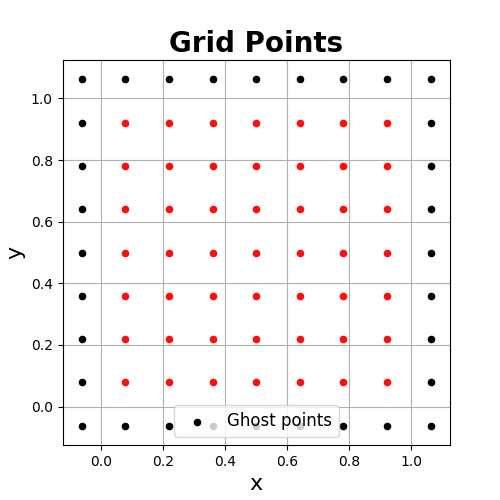
\includegraphics[width=0.5\textwidth]{grid.png}
				\caption{Grid layout}
		\end{figure}
		
		\pagebreak
	\section{Comparison with Exact Solution, Dirichlet Boundary Conditions}
		Given the exact solution:
		$$u_{ex}\left(x,y\right) = \sin\left(2\pi n x\right)\sin\left(2\pi n y\right)$$
		and homogeneous Dirichlet boundary conditions, the Poisson equation was solved for a
		range of values
		of $n$ that met the Nyquist criterion.  Plots of the exact solution can be seen in
		figures 2-4.

		\begin{figure}[h]
			\centering
				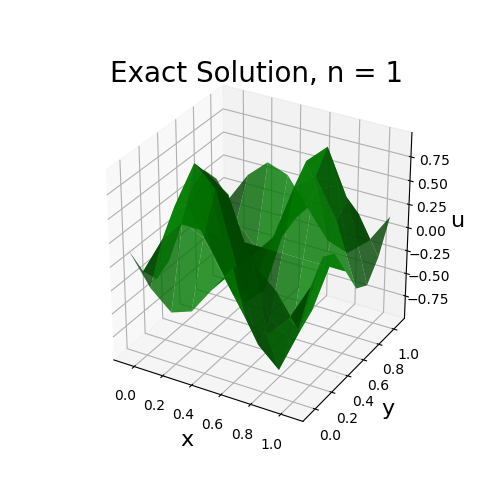
\includegraphics[width=0.5\textwidth]{exn1.png}
				\caption{Exact solution with $n=1$}
		\end{figure}

		\begin{figure}[h]
			\centering
				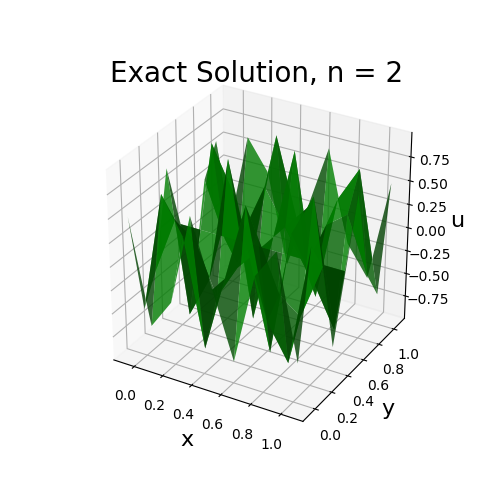
\includegraphics[width=0.5\textwidth]{exn2.png}
				\caption{Exact solution with $n=2$}
		\end{figure}

		\begin{figure}[h]
			\centering
				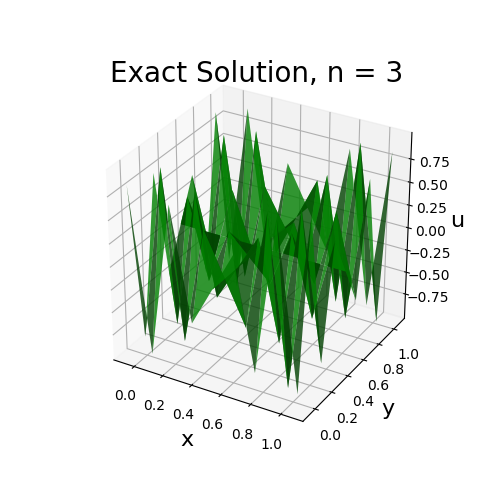
\includegraphics[width=0.5\textwidth]{exn3.png}
				\caption{Exact solution with $n=3$}
		\end{figure}

		\subsection{Jacobi Method}
			First,  a  mesh grid was created to represent the $x$ and $y$ domains.  A simple $9$ by
			$9$ grid was used for the first section, as grid refinement would come later.  Plots of
			the results can be seen in figures 5-7.

			\begin{figure}[h]
				\centering
					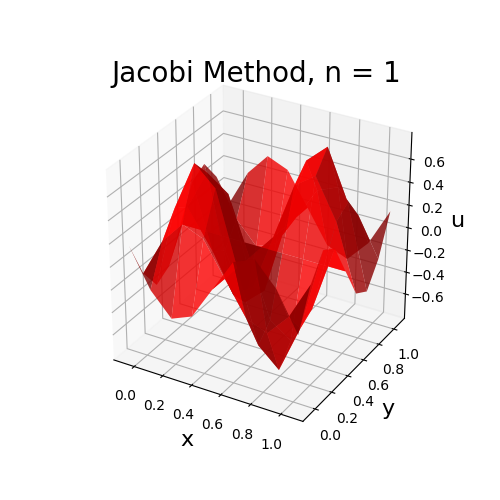
\includegraphics[width=0.5\textwidth]{jmn1.png}
					\caption{Jacobi method with $n=1$}
			\end{figure}

			\begin{figure}[h]
				\centering
					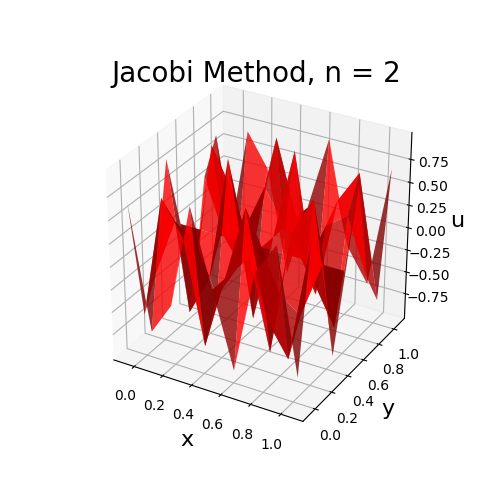
\includegraphics[width=0.5\textwidth]{jmn2.png}
					\caption{Jacobi method with $n=2$}
			\end{figure}

			\begin{figure}[h]
				\centering
					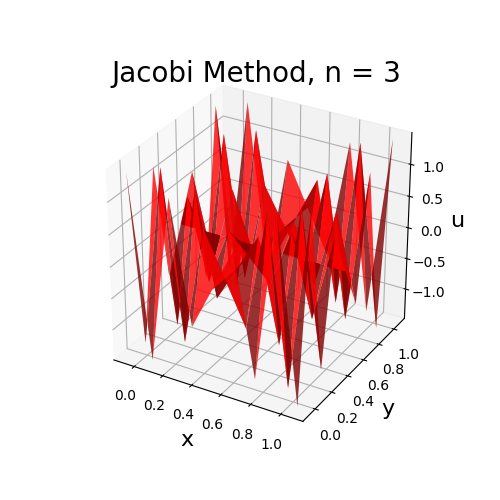
\includegraphics[width=0.5\textwidth]{jmn3.png}
					\caption{Jacobi method with $n=3$}
			\end{figure}

		\subsection{Successive Over Relaxation (SOR)}
			The same mesh grid was created yet again, and a relaxation parameter
			$\omega=\frac{2}{2 - cos{\left(2\pi \Delta x\right)}}$ was assigned.  Plots of the results may be seen in figures 8-10.

			\begin{figure}[h]
				\centering
					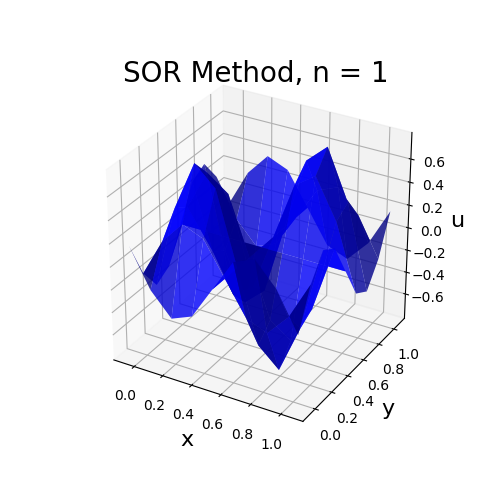
\includegraphics[width=0.5\textwidth]{sorn1.png}
					\caption{Gauss-seidel method with SOR, $\omega=1.1$, $n=1$}
			\end{figure} 

			\begin{figure}[h]
				\centering
					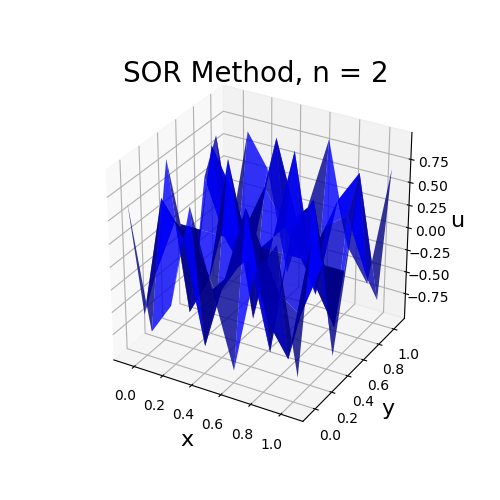
\includegraphics[width=0.5\textwidth]{sorn2.png}
					\caption{Gauss-seidel method with SOR, $\omega$, $n=2$}
			\end{figure} 

			\begin{figure}[h]
				\centering
					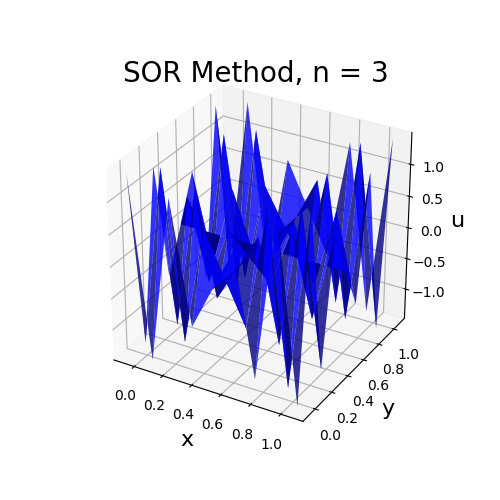
\includegraphics[width=0.5\textwidth]{sorn3.png}
					\caption{Gauss-seidel method with SOR, $\omega$, $n=3$}
			\end{figure}
			
			\pagebreak
			
	\section{Grid Refinement Study}
		Next, a grid refinement study was performed using a range of grid sizes from $5$ by
		$5$ to $513$ by $513$.  A plot of the results can be seen in figure 11.
		
		\begin{figure}[h]
			\centering
				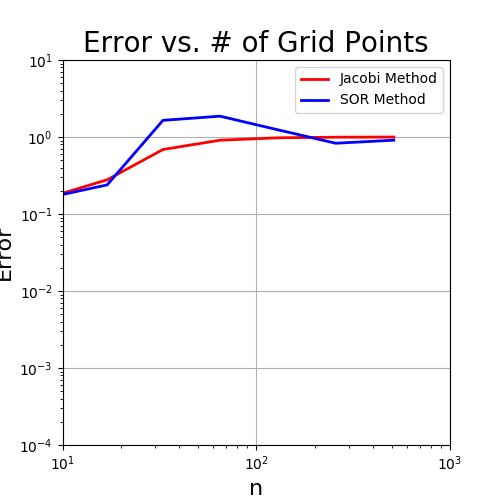
\includegraphics[width=0.5\textwidth]{grid_refine.png}
				\caption{Grid refinement results for both methods used}
		\end{figure}
		
		\pagebreak
	\section{Neumann Boundary Conditions}
		A new exact solution,
		$$u_{ex}\left(x,y\right) = cos{\left(2\pi nx\right)cos\left(2\pi nx\right)}$$
		was given with Neumann boundary conditions.  Both methods were used again, and another grid
		refinement study was performed.  Results can be seen in figures 12-21.
		
\end{document}